\chapter{Tecniche di enumerazione}

\section{Cardinalità degli insiemi}

\subsection{Il principio di inclusione-esclusione}
Vogliamo contare il numero di elementi dell'unione di due o più insiemi finiti. In teoria insiemistica, per indicare il numero di elementi di un insieme finito $A$ si usa il simbolo $|A|$, tale numero indica la \textbf{cardinalità}, ovvero il numero di elementi, dell'insieme $A$. Iniziamo col caso di due insiemi.

\begin{propbox}
	Siano $A$ e $B$ due insiemi finiti di cardinalità finita $n$ e $m$ rispettivamente, che siano disgiunti ($A \cap B = \varnothing$). Allora
	\begin{equation}
		|A \cup B| = |A| + |B| = n+m
	\end{equation}
\end{propbox}

La formula si generalizza al caso di $k$ insiemi finiti $A_{i}$, $i=1,2,\ldots, k$, con $|A_{i}|=n_{i}$, disgiunti due a due:
\begin{equation}
	|\bigcup A_{i}| = \sum_{i=1}^{k} |A_{i}| = n_{i} + \ldots + n_{k}
\end{equation}

\begin{propbox}[Principio di inclusione-esclusione]
	Siano $A$ e $B$ due insiemi finiti con $k$ elementi in comune, ossia $k=|A \cap B|$, allora:
	\begin{equation}\label{eq:pie}
		|A \cup B| = |A| +|B| - |A \cap B| = n+m-k
	\end{equation}
\end{propbox}
Il termine correttivo $-k$ si inserisce poiché i $k$ elementi comuni ad $A$ e $B$ compaiono tra gli $n$ del primo insieme e gli $m$ del secondo e sarebbero pertanto contati due volte in $n+m$. Tralasciamo la sua generalizzazione al caso di $k$ insiemi poiché decisamente più complicata. La riportiamo solo per il caso $k=3$:
\begin{equation}\label{eq:pie2}
	|A_{1}+A_{2}+A_{3}| = |A_{1}|+|A_{2}|+|A_{3}| - |A_{1} \cap A_{2}| - |A_{1} \cap A_{3}|- |A_{2} \cap A_{3}|- |A_{1} \cap A_{2} \cap A_{3}|
\end{equation}

\begin{example}
	Su 25 studenti, 15 hanno superato l'esame di Analisi, 12 quello di Programmazione e 5 hanno superato entrambi gli esami. Quanti studenti hanno superato almeno un esame? Quanti studenti hanno fallito entrambi gli esami? Sia $A$ l'insieme degli studenti che hanno superato l'esame di Analisi: $|A|=15$. Sia $B$ l'insieme degli studenti che hanno superato l'esame di Programmazione, $|B|=12$. $A \cap B$ è l'insieme degli studenti che hanno superato entrambi gli esami: $|A \cap B|=5$. La risposta alla prima domanda è l'ordine dell'insieme $A \cup B$, dato da $15+12-5=22$. Non hanno superato nessuno dei due esami $25-22=3$ studenti.
\end{example}

\begin{example}
	Sia $I=\{1,2,\ldots,20\}$. Quanti sono i numeri di $I$ divisibili per 2 o per 3? Sia $A$ l'insieme dei numeri pari di $I$: l'ordine di $A$ è 10. Sia $B$ l'insieme dei multipli di 3 in $I$: $B=\{3,6,9,12,15,18\}$ ha ordine 6. $A \cap B$ è l'insieme dei multipli di 6 minori di 20: $A \cap B = \{6,12,18\}$ ha ordine 3. I numeri di $I$ divisibili per due o per 3 sono $10+6-3=13$.
\end{example}

\begin{example}
	In un gruppo di amici  tutti hanno visto almeno uno dei film $x,\ y,\ z$: 8 hanno visto il film $x$, 12 il film $y$ e 9 il film $z$. Inoltre 6 hanno visto $x$ e $y$, 4 hanno visto $x$ e $z$, 7 hanno visto $y$ e $z$ e soltanto uno di essi ha assistito alle tre proiezioni. Da quante persone è formato il gruppo? Con ovvio significato delle notazioni si ha: $\lvert X \rvert = 8$, $\lvert Y \rvert = 12$ , $ \lvert Z \rvert = 9 $, $\vert X \cap Y\vert = 6$, $\vert X \cap Z\vert = 4$, $\vert Y\cap Z\vert = 7$, $\lvert X\cap Y\cap Z\vert = 1$. Quindi:
	\begin{displaymath}
		\lvert X \cup Y \cup Z \rvert = 8+12+9-4-7+1=13
	\end{displaymath}
\end{example}
\subsection{Insiemi finiti}

\begin{propbox}\label{prop:cardinalità_prodotto_Cartesiano}
	Siano $A$ e $B$ insiemi non vuoti tali che $|A|=n$ e $|B|=m$. Allora il prodotto cartesiano $A \times B$ avrà precisamente $nm$ elementi:
	\begin{equation}
		|A \times B| = nm
	\end{equation}
\end{propbox}


\begin{proof}
	Se $A={a_{1},...,a_{n}}$, consideriamo gli $n$ sottoinsiemi $B_{i}$ di $A \times B$ a due a due disgiunti formati ognuno dalle $m$ coppie aventi $a_{i}$ come prima componente. Si avrà quindi:
	\begin{displaymath}
		|A \times B| = |B_{1}|+\cdots + |B_{n}|=nm
	\end{displaymath}
\end{proof}


\begin{lemmabox}
	Siano $A$ e $B$ insiemi non vuoti tali che $|B|=m$ e $|A|=n$. Il numero di applicazioni $A \longrightarrow B$ è $m^{n}$:
	\begin{equation}\label{eq:mapab}
		|Map(A,B)| = m^{n}
	\end{equation}
	In teoria degli insiemi si denota l'insieme $Map(A,B)$ col simbolo $B^{A}$. Quindi:
	\begin{equation}
		|B^{A}|=|B|^{|A|}=m^{n}
	\end{equation}
\end{lemmabox}
\begin{proof}
	Poniamo $A=\{a_{1},a_{2},\ldots,a_{n}\}$. Preso un $\overline{a} \in A$ esistono $m$ possibili scelte come sua immagine, possiamo quindi dire che un'applicazione $f: a \rightarrow B$  è univocamente determinata dalla $n$-pla delle immagini $(f(a_{1}),f(a_{2}),\ldots,f(a_{n})) \in B^{n}$, dove $B^{n}$ è il prodotto cartesiano di $B$ con se stessa per $n$ volte.  Sfruttando la Proposizione \ref{prop:cardinalità_prodotto_Cartesiano} sappiamo che $|B^{n}| = \underbrace{m \cdot \ldots \cdot  m}_{\text{$n$ volte}} = m^{n}$. Quindi $|B^{A}| = |B^{n}| =  m^{n}$.
\end{proof}
\begin{example}
	Dato un alfabeto $C$ di $k$ caratteri, quante parole (stringhe) di lunghezza $n$ sull'alfabeto $C$ esistono? La domanda si traduce nella ricerca di tutte le possibili applicazioni dall'insieme $I_{n} = \{1,2,3,\ldots,n\}$ all'insieme $C$. Infatti una stringa di lunghezza $n$ può essere espressa nella forma:
	\[
	\bigl[g(1) \ g(2) \ g(3) \ \ldots \ g(n) \bigr]
	\]
	con $g \in Map(I_{n},C)$. Per il lemma precedente abbiamo quindi $|Map(I_{n},C)| = k^{n}$ possibili stringhe.
\end{example}
\begin{example}
	Sia $A=\{a_{1},a_{2},a_{3}\}$ e $B=\{b_{1},b_{2}\}$. Abbiamo quindi che $|A|=3$, $|B|=2$ e $|Map(A,B)|=2^{3}=8$. Per trovare tutte le otto applicazioni da $A$ in $B$ basta costruire la seguente tabella:
	\begin{center}
		\begin{tblr}
			{
				hline{1-Z} = {0.9pt},
				vline{1-Z} = {0.9pt},
				vline{1} = {1}{0pt},
				hline{1} = {1}{0pt},
				cells={mode=math},
				cell{1}{2-Z}={primary!40!white},
				cell{2-Z}{1}={primary!40!white}
			}
			& f_{0} & f_{1} & f_{2} & f_{3} & f_{4} & f_{5} & f_{6} & f_{7} \\
			a_{1} &b_{1} & b_{1}& b_{1}& b_{1}& b_{2}& b_{2}& b_{2}&b_{2}\\
			a_{2} &b_{1} & b_{1}& b_{2}& b_{2}& b_{1}& b_{1}& b_{2}&b_{2}\\
			a_{3} &b_{1} & b_{2}& b_{1}& b_{2}& b_{1}& b_{2}& b_{1}&b_{2}\\
		\end{tblr}
		\captionof{table}{Elementi di $Map(A,B)$}
	\end{center}
	In questo caso troviamo due applicazioni costanti ($f_{0},f_{7}$), le applicazioni $f_{1:6}$ sono suriettive mentre nessuna applicazione è iniettiva.
\end{example}

In generale, la presenza o meno di applicazioni iniettive in $B^{A}$ dipende dalla relazione $n\leq m$. Non a caso, nel caso analizzato nell'esempio precedente, non esistevano applicazioni iniettive in quanto $|A|=3>2=|B|$. Si consideri l'insieme $A=\{a_{1}, a_{1},...,a_{n}\}$. Una applicazione $f$ per essere iniettiva deve associare $n$ valori diversi a ciascun elemento di $A$ quindi la cardinalità del suo codominio deve essere \textit{almeno pari} a quella del dominio $A$.

\begin{propbox}[Condizione esistenza applicazioni iniettive]\label{prop:esistenza_iniettive}
	Esistono applicazioni iniettive in $B^{A}$ se e solo se:
	\begin{equation}
		|A| \leq |B|
	\end{equation}
	nel caso, il loro numero è dato da:
	\begin{equation}\label{eq:injmap}
		|Inj \ Map(A,B)|= m(m-1)(m-2)\cdots(m-n+1)=m^{\underline{n}}
	\end{equation}
	dove $m^{\underline{n}}$ è chiamato \textbf{fattoriale discendente\footnote{Notazione introdotta da Donald Knuth. Conosciuto per essere l'autore di \textit{The Art of Computer Programming}, è considerato il padre del campo di studio che studia in maniera rigorosa la parte algoritmica della teoria della complessità e ha dato fondamentali contributi in svariati rami dell'informatica teorica.}}.
\end{propbox}

\begin{proof}
	Consideriamo gli insiemi $A=\{a_{1},...,A_{n}\}$ e $B=\{b_{1},...,b_{m}\}$ per costruire una applicazione iniettiva da $A$ in $B$ possiamo procedere nel modo seguente. Preso $a_{1}\in A$ esistono $m$ possibili scelte in $B$ da far mappare su $a_{1}$:
	\begin{displaymath}
		a_{1} \mapsto \mbox{... $m$ scelte possibili in $B$}
	\end{displaymath}
	passando all'elemento $a_{2}$ non avremo più $m$ possibili scelte bensì $m-1$ per garantire l'iniettività dell'applicazione che stiamo costruendo:
	\begin{displaymath}
		a_{2} \mapsto \mbox{... $m-1$ scelte possibili in $B$}
	\end{displaymath}
	procedendo in avanti:
	\begin{displaymath}
		a_{3} \mapsto \mbox{... $m-2$ scelte possibili in $B$}
	\end{displaymath}
	
	Se $n>m$ chiaramente non sarà possibile trovare nuovi elementi distinti da mappare per ogni elemento $a_{i}$, non sarà possibile quindi costruire una applicazione iniettiva. Nel caso contrario, se $n \leq m$, anche all'elemento $a_{n}$ sarà possibile mappare un elemento distinto da tutti gli altri precedentemente selezionati e in particolare:
	\begin{displaymath}
		a_{n} \mapsto \mbox{... $m-(n-1)$ scelte possibili in $B$}
	\end{displaymath}
	Dove $m-(n-1)$ sarà sicuramente maggiore di zero in quanto $n\leq m$. Per l'$i$-esimo elemento di $A$ esisteranno quindi, sotto questa condizione, $m-i+1$ possibili scelte in $B$ da mappare:
	\begin{displaymath}
		a_{i} \mapsto \mbox{... $m-i+1$ scelte possibili in $B$}
	\end{displaymath}
	L'insieme delle coppie ordinate così costruite sarà quindi composto da:
	\begin{displaymath}
		m(m-1)(m-2)\cdots(m-n+1)
	\end{displaymath}
	elementi.
\end{proof}

\begin{example}
	Si consideri l'insieme delle lettere dell'alfabeto italiano:
	\begin{displaymath}
		I = \{A,B,C,D,E,F,G,H,I,L,M,N,O,P,Q,R,S,T,U,V,Z\}
	\end{displaymath}
	Cercare stringhe di lunghezza 5 in cui non ci siano ripetizioni significa cercare le applicazioni iniettive dall'insieme delle posizioni $P=\{1,2,3,4,5\}$ all'insieme $I$. Il numero di applicazioni iniettive che possiamo costruire sarà:
	\begin{displaymath}
		21^{\underline{5}}=21 \cdot 20 \cdot 19 \cdot 18 \cdot 17 =2441880
	\end{displaymath}
\end{example}


\begin{corolbox}
	È possibile riscrivere l'equazione \ref{eq:injmap} in termini di fattoriale e vale:
	\begin{equation}
		|Inj \ Map(A,B)| = \frac{m!}{(m-n)!}
	\end{equation}
\end{corolbox}

\begin{defbox}{Equipotenza}
	Due insiemi $A$ e $B$ si dicono \textbf{equipotenti}\index{Equipotenza} se e solo se:
	\begin{equation}
		|A|=|B|
	\end{equation}
\end{defbox}

\gbox{Principio della piccionaia}{green!80!black}{
	Se una piccionaia ha $m$ nicchie e $n$ piccioni, con $n>m$, allora almeno due piccioni finiscono nella stessa nicchia.
}

Tradotto in termini rigorosi, il principio sostiene che, se $n>m$, nessuna funzione di $A$ in $B$ è iniettiva. Più in generale vale quanto segue:

\begin{teorbox}
	Dati $A$ e $B$ insiemi finiti. Assumiamo $|A|=n$ e $|B|=m$. Allora:
	\begin{enumerate}
		\item Esistono applicazioni iniettive da $A$ in $B$ se e soltanto se $n \leq m$;
		\item Esistono applicazioni suriettive da $A$ in $B$ se e soltanto se $n \geq m$ oppure se da $B = \varnothing$ allora  segue $ A = \varnothing$.
		\item Esistono applicazioni biettive da $A$ in $B$ se e soltanto se i due insiemi sono equipotenti, cioè $n=m$;
	\end{enumerate}
\end{teorbox}

\begin{proof}
	Si ha:
	\begin{enumerate}
		\item Già vista nella proposizione \ref{prop:esistenza_iniettive}.
		\item Sia $B \neq \varnothing$ e sia $m \leq n$, esiste quindi una applicazione iniettiva $f: B \rightarrow A$. In questo caso esiste sicuramente una retrazione di $f$, ovvero una applicazione $h: A \rightarrow B$ che è sicuramente suriettiva. 
		
		Viceversa, se esiste un'applicazione $f:A \rightarrow B$ suriettiva allora $f$ ammette sezioni $h:B \rightarrow A$ e tale applicazione è iniettiva e vale $|A| \geq |B|$. Se $B$ è l'insieme vuoto esistono invece due casi:
		\begin{itemize}
			\item Se $n>0$ allora non esistono applicazioni da $A$ in $B$;
			\item Se $n=0$ allora $A=B=\varnothing$ e $B^{A}= Map(A,B)=\{id_{\varnothing}\}$ che risulta biettiva, e in particolare suriettiva.
		\end{itemize}
		\item  Se esistono applicazioni biettive da $A \longrightarrow B$ allora esistono applicazioni che siano iniettive e suriettive, quindi $n \leq m \land m \leq n \implies n=m$ e i due insiemi risultano equipotenti. Viceversa, siano $A$ e $B$ equipotenti. Ponendo $f(a_{i})=b_{i}$ per ogni $i=1,...,n$ si definisce una funzione biettiva di $A$ in $B$.
	\end{enumerate}
\end{proof}

\begin{corolbox}
	Siano $A$ e $B$ due insiemi finiti. Allora: 
\begin{equation}
		|A|\leq |B| \land  |B| \leq |A| \implies |A|=|B|
\end{equation}
\end{corolbox}

\begin{teorbox}
	Siano $A$ e $B$ due insiemi finiti equipotenti e sia $f:A \rightarrow B$ un'applicazione. Allora sono equivalenti:
	\begin{enumerate}
		\item $f$ è iniettiva
		\item $f$ è suriettiva
		\item $f$ è biettiva
	\end{enumerate}
\end{teorbox}

\begin{proof}
	\begin{itemize}
		\item Consideriamo l'immagine di $f$, l'insieme $im \ f = \{f(x) \; | \; x \in A\}$. Siccome $f$ è iniettiva, $im \ f$ ha la stessa cardinalità di $A$ perché ad ogni elemento di $A$ corrisponde un elemento distinto in $im \ f$. Ora, dato che $A$ è equipotente a $B$, la cardinalità di $A$ è uguale a quella di $B$. Quindi, la cardinalità di $im \ f$ è uguale a quella di $B$ per transitività. Poiché $im \ f \subseteq B$ e $|im \ f| = |B$, l'unica possibilità è che $im \ f = B$, ma ciò significa che $f$ è suriettiva, e quindi biettiva. Quindi $(1 \implies 3)$.
		\item Che $(3 \implies 2)$ risulta ovvio.
		\item Resta da dimostrare che $(2 \implies 1)$. Supponiamo che $f$ sia suriettiva. Allora $f$, per il Teorema \ref{thm:car_sezioni}, ha una sezione $g: B \rightarrow A$, ovviamente $g$ risulta iniettiva (in quanto, per definizione di sezione, deve essere $f \circ g = id_{B}$ ed $f$ risulta essere una retrazione per $g$. Avendo dimostrato che se $f$ è una applicazione iniettiva tra due insiemi equipotenti allora questa risulta essere una biezione, allora $g$ è una applicazione biettiva e quindi invertibile. Applicando i risultati del Teorema \ref{thm:unicità_inversa} $f$ è l'unica retrazione di $g$ e coincide con la sua inversa. Allora $f = g^{-1}$ che risulta essere biettiva. e in particolare iniettiva. Come volevasi dimostrare.
	\end{itemize}
\end{proof}

\begin{corolbox}
	Se $|A| = |B|=m$ allora ogni applicazione iniettiva da $A$ a $B$ è biettiva. In questo caso:
	\begin{displaymath}
		|Inj \ Map(A,B)| = \frac{|a|!}{(|a|-|b|)|}= \frac{|a|!}{0!}=m!
	\end{displaymath}
\end{corolbox}

\begin{osservation}
	Per le conclusioni appena dimostrate, un insieme risulta infinito se esiste un'applicazione iniettiva $f: A \rightarrow A$. Inoltre, l'insieme delle permutazioni in un insieme $A$, $Sym(A)$, ovvero l'insieme delle applicazioni biettive $\sigma: A \longrightarrow A$ ha ben $|A|!$ elementi.
\end{osservation}

\begin{example}
	Sono equipotenti l'insieme $\mathbb{N}$ dei numeri naturali e l'insieme $\mathbb{Z}$ dei numeri interi relativi. Consideriamo infatti la funzione:
	\begin{displaymath}
		h: n \in \mathbb{N} \mapsto \begin{cases}
			\frac{n}{2} & \text{se $n$ è pari} \\
			-\frac{n+1}{2} & \text{se $n$ è dispari}
		\end{cases}
		\in \mathbb{Z}
	\end{displaymath}
	Chiaramente $h$ è iniettiva, infatti:
	\begin{align*}
		\forall a,b \in \mathbb{N} \bigl(h(a)=h(b) \implies a=b\bigr)
	\end{align*}
	Se $h(a)=h(b)$ possiamo avere i due seguenti casi:
	\begin{align*}
		\begin{cases}
			\frac{a}{2} = \frac{b}{2} \implies a= b \\
			-\frac{a+1}{2} = -\frac{b+1}{2} \implies a=b
		\end{cases}
	\end{align*}
	Inoltre, per ogni $b \in \mathbb{Z}$ possiamo trovare un elemento $x \in \mathbb{N}$ per il quale valga $b=h(x)$:
	\begin{itemize}
		\item Se $b \in \mathbb{N}$ allora $b=h(2b)$;
		\item Se $b \in \mathbb{Z}\setminus \mathbb{N}$ allora $b=h(-2b-1)$.
	\end{itemize}
	Ciò dimostra la suriettività di $h$ che risulta infine biettiva. L'inversa della funzione $h$ è:
	\begin{displaymath}
		h^{-1}: b \in \mathbb{Z} \mapsto \begin{cases}
			2b & \text{se } b \geq 0 \\
			2b-1 & \text{se } b <0
		\end{cases} \in \mathbb{N}
	\end{displaymath}
	Quindi $|\mathbb{N}|=|\mathbb{Z}|$.
\end{example}

\begin{defbox}{Insiemi infiniti}
	Un insieme è \textbf{infinito} se è equipotente ad un suo sottoinsieme
	proprio. Un insieme è \textbf{finito} se questo non capita.
\end{defbox}

\begin{example}
	L'insieme dei numeri naturali $\mathbb{N}$ è un insieme infinito poiché la funzione ``successore'' $\sigma: \mathbb{N} \rightarrow \mathbb{N}$, $\sigma(n) = n+1$ è iniettiva ma non suriettiva. Possiamo anche vedere che la funzione ``doppio'' $f: \mathbb{N} \rightarrow P$ (dove $P$ è l'insieme dei numeri pari) data da $f(n)=2n$ è biunivoca e quindi $\mathbb{N}$ è equipotente ad una sua parte propria.
\end{example}

\subsection{La funzione caratteristica e la cardinalità dell'insieme delle parti}

\begin{defbox}{Funzione caratteristica}\index{Funzione caratteristica}
	Sia $S$ un insieme e $T\subseteq S$ un suo sottoinsieme. L'applicazione $\mbox{\Large$\chi$}_{T,S} \in Map(S, \{0,1\})$, definita come:
	\begin{equation}
		\mbox{\Large$\chi$}_{T,S} : x \in S \mapsto \begin{cases}
			1 & \text{se } x \in T \\
			0 & \text{se } x \notin T
		\end{cases} \in \{0,1\}
	\end{equation}
	prende il nome di \textbf{applicazione caratteristica}\footnote{Può essere visto come un predicato logico che verifica l'appartenenza di un elemento $x$ in $T$} di $T$ in $S$.
\end{defbox}

\begin{example}
	Sia $S=\{1,2,3,4,5,6,7\}$ e sia $T = \{2,4,7\} \in \mathcal{P}(S)$, allora $\mbox{\Large$\chi$}_{T,S}$ è uguale a:
	\[
	\left\lgroup
	\begin{array}{ccccccc}
		1 & 2 & 3 & 4 & 5 & 6 & 7 \\
		0 & 1 & 0 & 1 & 0 & 0 & 1
	\end{array}
	\right\rgroup
	\]
\end{example}

Si considerino le applicazioni biettive:
\begin{displaymath}
	\begin{array}{l}
		\alpha: T \in \mathcal{P}(S) \mapsto \mbox{\Large$\chi$}_{T,S} \in M \\
		\beta: f \in Map(S,\{0,1\}) \mapsto \overleftarrow{f}(\{1\}) \in \mathcal{P}(S)
	\end{array}
\end{displaymath}
allora vale il seguente teorema:



\begin{teorbox}
	Le applicazioni biettive $\alpha$ e $\beta$  sono l'una l'inversa dell'altra.
\end{teorbox}

\begin{proof}
	Per comodità poniamo $M=Map(S,\{0,1\})$. Per dimostrare l'enunciato bisogna verificare che $\beta$ sia una sezione ed una retrazione di $\alpha$ ovvero:
	\begin{displaymath}
		\begin{array}{l}
			\alpha \circ \beta = id_{M}\\
			\beta \circ \alpha = id_{\mathcal{P}(S)}
		\end{array}
	\end{displaymath}
	\begin{enumerate}
		\item Si ha chiaramente che, per ogni applicazione $f \in M$:
		\begin{align*}
			\alpha(\beta(f)) &=\alpha\bigl(\overleftarrow{f}(\{1\})\bigl) \\
			& = \mbox{\Large$\chi$}_{\overleftarrow{f}(\{1\}),S} \mapsto \begin{cases}
				1 & \text{se } x \in \overleftarrow{f}(\{1\})\\
				0 & \text{se } x \notin \overleftarrow{f}(\{1\})
			\end{cases}
		\end{align*}
		e si ha che, $\forall x \in S$:
		\begin{displaymath}
			x \in \overleftarrow{f}(\{1\}) \iff f(x) \in \{1\} \iff f(x)=1
		\end{displaymath}
		dunque, per ogni $f \in M$,
		\[\mbox{\Large$\chi$}_{\overleftarrow{f}(\{1\}),S}: x \in S \mapsto \begin{cases}
			1 & \text{ se } f(x) = 1 \\
			0 & \text{ se } f(x) = 0 \\
		\end{cases}
		\]
		il che è equivalente a mappare $x \in S$ su $f(x) \in \{0,1\}$, quindi $\mbox{\Large$\chi$}_{\overleftarrow{f}(\{1\}),S} = f$ e abbiamo $\alpha(\beta(f)) = f$, cioè $\alpha \circ \beta= id_{M}$.
		\item Per ogni sottoinsieme $T$ di $S$, si ha:
		\begin{align*}
			\beta\bigl(\alpha(T)\bigl) = \beta(\mbox{\Large$\chi$}_{T,S}) = \overleftarrow{\mbox{\Large$\chi$}_{T,S}}(\{1\}) = \{x \in S \; | \; \mbox{\Large$\chi$}_{T,S}(x) = 1\} = T
		\end{align*}
		Quindi $\beta \circ \alpha = id_{\mathcal{P}(S)}$ e l'enunciato è dimostrato. 
	\end{enumerate}
\end{proof}


\begin{corolbox}
	Se $S$ è un insieme finito con $n$ elementi allora avrà esattamente $2^{n}$ parti finite. Ovvero:
	\begin{equation}
		|\mathcal{P}(S)| = |Map(S,\{0,1\})|= 2^{|S|}=2^{n}
	\end{equation}
\end{corolbox}

\begin{proof}
	Basta applicare la formula \ref{eq:mapab} e osservare che $|\{0,1\}|=2$. 
\end{proof}

\begin{defbox}{Coefficiente binomiale}\index{Coefficiente binomiale}
	Dati $S$ un insieme di $n$ elementi e $k \in \mathbb{N}$ è possibile considerare l'insieme:
	\begin{equation}
		\mathcal{P}_{k}(S)= \{X \subseteq S \; | \; |X| = k\}
	\end{equation}
	ovvero l'insieme delle parti di $S$ con $k$ elementi. Per indicare la cardinalità di $\mathcal{P}_{k}(S)$ si usano i \textbf{coefficienti binomiali}. Ovvero:
	\begin{equation}
		\binom{n}{k} = |\mathcal{P}_{k}(S)|
	\end{equation}
	dove $\binom{n}{k}$ si legge ``coefficiente binomiale di $n$ su $k$''.
\end{defbox}


\begin{osservation}
	Alcuni coefficienti binomiali immediati da calcolare: per ogni $n \in \mathbb{N}$ vale:
	\begin{equation}
		\binom{n}{0} = 1 = \binom{n}{n}
	\end{equation}
	Infatti, se consideriamo un insieme finito $S$ di cardinalità $n$, il numero di sottoinsiemi di cardinalità pari a zero è uno in quanto il solo insieme vuoto risulta avere tale cardinalità. Analogamente, l'unico sottoinsieme di $S$ di cardinalità pari a quella di $S$ risulta $S$ stesso.  Un'altra proprietà molto semplice da verificare è:
	\begin{equation}
		\binom{n}{1} = n
	\end{equation}
	La cui dimostrazione è abbastanza banale in quanto in un insieme finito di $n$ elementi esistono sempre $n$ singleton.
\end{osservation}

\begin{propbox}
	Per ogni $n \in \mathbb{N}$ si ha:
	\begin{equation}
		\sum_{k=0}^{n} \binom{n}{k} = 2^{n}
	\end{equation}
\end{propbox}

\begin{proof}
	Sia $S$ un insieme tale che $|S|=n$. È chiaro che $\mathcal{P}(S)$ è unione disgiunta degli insiemi $\mathcal{P}_{k}(S)$ al variare dell'intero $k$ tra $0$ ed $n$. In altri termini $\{\mathcal{P}_{k}(S) \; | \; k \in \mathbb{N} \land k \leq n \}$ è una partizione di $\mathcal{P}(S)$. Pertanto $\mathcal{P}(S)| = \sum_{k=0}^{n} \binom{n}{k} = 2^{n}$ e, per ogni scelta di $k$, $|\mathcal{P}_{k}(S)| = \binom{n}{k}$. Otteniamo così l'asserto.
\end{proof}

Si può pensare al coefficiente binomiale $\binom{n}{k}$ in questi termini: $\binom{n}{k}$ è il numero di modi in cui si possono scegliere $k$ oggetti da un insieme di $n$ oggetti (infatti scegliere $k$ oggetti significa in sostanza scegliere una $k$-parte). Ora, selezionare $k$ oggetti da un insieme di $n$ è concettualmente equivalente a sceglierne $n-k$ da scartare. Dunque dovrebbe essere facile comprendere che il coefficiente binomiale $\binom{n}{n-k}$ coincide con $\binom{n}{k}$.

\begin{propbox}
	Siano $n,k \in \mathbb{N}$ e sia $k \leq n$, vale allora:
	\begin{equation}
		\binom{n}{n-k} = \binom{n}{k}
	\end{equation}
\end{propbox}

\begin{proof}
	Consideriamo l'applicazione: 
	$$\xi: X \in \mathcal{P}(S) \mapsto S \setminus X \in \mathcal{P}(S)$$
	che ad ogni parte di $S$ associa il suo complemento in $S$.	Essendo $S \setminus (S \setminus X )= X$ ovvero $\xi(\xi(S \setminus X)) = \xi^{2}(S \setminus X) = X$ deve essere per forza $\xi^{2} = id_{\mathcal{P}(S)}$. 
	
	Per questo motivo $\xi$ corrisponde all'inversa di se stessa e dunque risulta essere biettiva. L'immagine dell'insieme $\mathcal{P}_{k}(S)$ è costituita dai complementi delle parti di $S$ con cardinalità pari a $k$. Tali complementi avranno cardinalità pari a $n-k$. Essendo $\xi$ una applicazione biettiva risulterà:
	\begin{displaymath}
		|\mathcal{P}_{k}(S)| = |\xi(\mathcal{P}_{k}(S)) | = |\mathcal{P}_{n-k}(S)|
	\end{displaymath}
	da cui deriva l'asserto. 
\end{proof}

\begin{propbox}
	Sia $n,k \in \mathbb{N}$ vale allora:
	\begin{equation}\label{eq:binom}
		\binom{n+1}{k+1} = \binom{n}{k+1} + \binom{n}{k}
	\end{equation}
\end{propbox}

\begin{proof}
	Diamo questa dimostrazione in una versione poco formalizzata ma più facile da seguire di quanto sarebbe in una stesura più rigorosa.
	
	Supponiamo di avere un insieme $S$ costituito da $n + 1$ palline bianche. Ovviamente $S \neq \emptyset$, perché $n+1>0$, quindi possiamo selezionare una delle palline e colorarla, diciamo, di nero. Il coefficiente binomiale che vogliamo calcolare, $\binom{n+1}{k+1}$, è il numero delle $k+1$ parti di $S$. Possiamo distinguere tra due tipi di $(k+1)$-parti di $S$: quelle costituite da sole palline bianche e quelle costituite dalla pallina nera e da $k$ palline bianche. Ovviamente $\binom{n+1}{k+1}$ è la somma tra il numero delle parti del primo tipi ed il numero delle parti del secondo tipo. Quante sono le parti del primo tipo? Esse sono precisamente le $(k+1)$-parti dell'insieme delle palline bianche. Poiché il numero delle palline bianche è $n$, questo numero sarà $\binom{n}{k+1}$. Quante sono invece le parti del secondo tipo? Ciascuna di esse si ottiene aggiungendo la pallina nera del secondo tipo ad una $k$-parte dell'insieme delle palline bianche, e da ciò è facile dedurre che il numero delle parti del secondo tipo è uguale a quello delle $k$ parti dell'insieme delle palline bianche, dunque $\binom{n}{k}$. Pertanto $\binom{n+1}{k+1}$, che come detto è uguale alla somma tra il numero delle parti del primo tipo ed il numero delle parti del secondo tipo, è proprio $\binom{n}{k+1} + \binom{n}{k}$, come volevasi dimostrare.
\end{proof}


	Questa proprietà permette di costruire i coefficienti binomiali con il cosiddetto \textbf{triangolo di Tartaglia} come mostrato in Figura \ref{fig:tartaglia}.



\begin{center}
	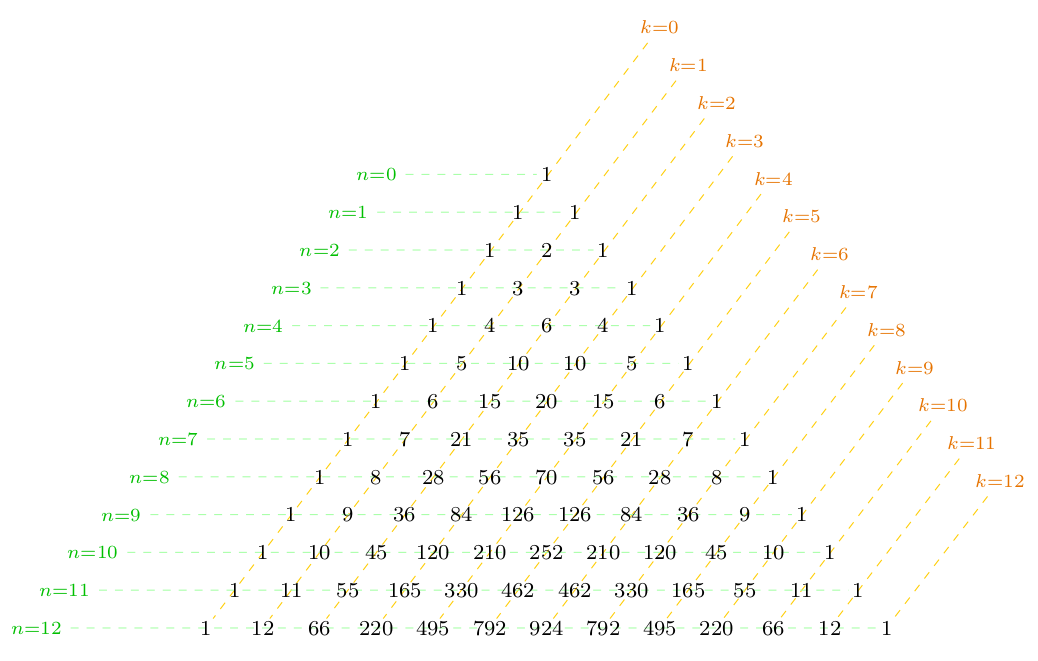
\includegraphics[scale=.5]{res/Tartaglia}
	\captionof{figure}{Triangolo di Tartaglia}\label{fig:tartaglia}
\end{center}

\section{Il principio di induzione}\label{sez:induzione}\index{Induzione}

\begin{propbox}[Principio di induzione (Prima forma)]
	Sia $p$ un predicato unario nella variabile $n$ e $b \in \mathbb{N}$ un numero naturale. Sia $\mathbb{N}_{b}=\{n \in \mathbb{N} \; | \; b \leq n \}$. Vale allora la seguente implicazione:
	\begin{equation}
		\Biggl(p(b) \land \Bigl(\forall n \in \mathbb{N}_{b}\bigl(p(n)\implies p(n+1) \bigr)\Bigr)\Biggr) \implies \forall n \in \mathbb{N}_{b} \bigl(p(n)\bigr)
	\end{equation}
	
\end{propbox}

\begin{proof}
	Si veda la sezione \ref{sez:buonordine}. 
\end{proof}

\begin{teorbox}
	Per ogni $n,k \in \mathbb{N}$ tali che $k \leq n$, vale allora:
	\begin{equation}
		\binom{n}{k} = \frac{n!}{k!(n-k)!}
	\end{equation}
\end{teorbox}

\begin{proof}
	Si dimostra per induzione.
	\begin{itemize}
		\item \textbf{Passo base:} sia $n=0$. Verifichiamo che il predicato sia vero. Se $n=0$ allora l'unico $k\leq n$ risulta essere $k=0$. Essendo $\binom{0}{0}=1$ allora  risulta :
		\begin{displaymath}
			\binom{0}{0} = \frac{0!}{0!} = 1
		\end{displaymath}
		e il predicato risulta vero. In generale:
		\begin{displaymath}
			\binom{n}{0} = \frac{n!}{0!(n-0)!} = \frac{n!}{n!} = 1
		\end{displaymath}
		\item \textbf{Passo induttivo:} assumiamo vero il predicato $p(n)$, dimostriamo $p(n) \implies p(n+1)$. Si ha:
		\begin{displaymath}
			\binom{n+1}{k} = \frac{(n+1)!}{k!(n+1-k)!}
		\end{displaymath}
		Se $k=0$ abbiamo che il predicato risulta vero. Se $k \neq 0$ applichiamo la formula \ref{eq:binom}:
		\begin{align*}
			\binom{n+1}{k} &= \binom{n}{k} + \binom{n}{k-1}\\
			&= \frac{n!}{k!(n-k)!} + \frac{n!}{(k-1)!(n-k+1)!}\\
			&= \frac{n!}{(k-1)!(n-k)!} \bigl(\frac{1}{k}+ \frac{1}{n-k+1}\bigr)\\
			&= \frac{n!}{(k-1)!(n-k)!} \bigl(\frac{n-k+1 +k}{k(n-k+1)}\bigr) \\
			&= \frac{n!(n+1)}{k!(n-k+1)!}\\
			&= \frac{(n+1)!}{k!\bigl((n+1)-k\bigr)!}
		\end{align*}
	\end{itemize}
	Il che dimostra il predicato $p(n+1)$.
\end{proof}
\newpage
\section{Esercizi svolti}
\begin{exsbox}
	Siano $X = \{1,2,3,4,5\}$ ed $Y=\{1,2,3\}$.
	\begin{enumerate}
		\item Quanti sono i sottoinsiemi di $X$ che contengono l'elemento 1?
		\item Quanti sono i sottoinsiemi $A$ di $X$ che contengono l'elemento 1 e tali che $A \cap \{2,3\} \neq \emptyset$?
		\item Quante sono le applicazioni iniettive da $X$ a $Y$?
		\item Quante sono le applicazioni iniettive da $Y$ a $X$?
		\item Quante sono le applicazioni suriettive da $X$ in $Y$?
	\end{enumerate}
\end{exsbox}
\paragraph{Svolgimento.} Abbiamo:
\begin{enumerate}
	\item Sia $\Omega$ l'insieme di tutti i sottoinsiemi di $X$ che contengono l'elemento $1$, ovvero:
	\begin{align*}
		\Omega \coloneqq \{A \subseteq X \; | \; 1 \in A\}
	\end{align*}
	Allora è immediato constatare che $\Omega$ è in corrispondenza biunivoca con l'insieme delle parti $X \setminus \{1\}$, mediante l'applicazione:
	\begin{align*}
		\varphi : \Omega \rightarrow \mathcal{P}(X \setminus \{1\})\\
		A \mapsto A \setminus \{1\}
	\end{align*}
	Ne segue che $|\Omega|= |\mathcal{P}(X \setminus \{1\})| = 2^{|X \setminus \{1\}|} = 2^{4} = 16$.
	\item Indichiamo con $\Theta$ il seguente insieme:
	\begin{align*}
		\Theta \coloneqq \{A \subseteq X \; | \; 1 \in A \land A \cap \{2,3\} \neq \emptyset \}
	\end{align*}
	Osserviamo che $\Theta$ è l'unione insiemistica di $\Lambda$ e $\Delta$, dove:
	\begin{align*}
		\Lambda \coloneqq \{ A \subseteq X \; | \; 1 \in A \land 2 \in A \}\\
		\Delta \coloneqq \{A \subseteq X \; | \; 1 \in A \land 3 \in A \}
	\end{align*}
	Pertanto $\Theta = \Lambda \cup \Delta$. Ragionando come nel punto precedente, si ha che:
	\begin{align*}
		|\Lambda|=|\Delta|= 2^{3} = 8
	\end{align*}
	Inoltre $\Lambda \cap \Delta \coloneqq \{A \subseteq X \; | \; \{1,2,3\} \subseteq A\}$, quindi $|\Lambda \cap \Delta|=2^{2}=4$. Siamo perciò in grado di calcolare con esattezza il numero di elementi di $\Theta$ tramite la \ref{eq:pie}:
	\begin{align*}
		|\Theta| = |\Lambda \cup \Delta| = |\Lambda|+|\Delta|-|\Lambda \cap \Delta| =12
	\end{align*}
	\item Essendo $|X| \geq |Y|$ non esistono applicazioni iniettive da $X$ in $Y$.
	\item Si ha $|Inj \ Map(Y,X)| = 5^{\underline{3}} = 5 \cdot 4 \cdot 3 = 60$ applicazioni iniettive.
	\item Sia $S \subseteq Map(X,Y)$ l'insieme di tutte le applicazioni suriettive da $X$ in $Y$. Inoltre, per ogni $y \in Y$ indichiamo con $A_{y}$ il sottoinsieme di $Map(X,Y)$ definito come:
	\begin{align*}
		A_{y} &\coloneqq \{f \in Map(X,Y) \; | \; y \notin f(X) \}\\
		&\coloneqq \{f \in Map(X,Y) \; | \; f^{-1}(\{y\}) = \emptyset\}
	\end{align*}
	Una applicazione $f$ è suriettiva se e solo se non appartiene a nessun $A_{y}$, per ogni $y=1,2,3$ abbiamo che:
	\begin{align}
		S = Map(X,Y) \setminus (A_{1} \cup A_{2} \cup A_{3})
	\end{align}
	Ne segue che:
	\begin{align*}
		|S| &=  |Map(X,Y)| - |A_{1} \cup A_{2} \cup A_{3}|\\
		&= 3^{5} - |A_{1} \cup A_{2} \cup A_{3}|
	\end{align*}
	Osserviamo che per ogni $f \in A_{1}$ vale $f(X) \subseteq \{2,3\}$, pertanto per tali funzioni l'insieme dei valori ammissibili è $\{2,3\}$, detto in altri termini: $|A_{1}| = |\{2,3\}|^{|X|} = 2^{5}$. Similmente per $A_{2}$ e $A_{3}$. Ora ci si accorge subito che $A_{1} \cap A_{2}$ contiene solo la funzione costante $c_{3}: x \mapsto 3$, per ogni $x \in X$ e, similmente, $A_{1} \cap A_{3} = \{c_{2}\}$, $A_{2} \cap A_{3} = \{c_{1}\}$. In particolare $|A_{1} \cap A_{2}|=|A_{1} \cap A_{3}| = |A_{2} \cap A_{3}| = 1$. Mentre $A_{1} \cap A_{2} \cap A_{3} = \emptyset$. Applicando la \ref{eq:pie2} otteniamo:
	\begin{align*}
		|A_{1} \cup A_{2} \cup A_{3}| &= |A_{1}|+|A_{2}| + |A_{3}| + |A_{1}\cap A_{2} \cap A_{3}| - |A_{1} \cap A_{2}| - |A_{1} \cap A_{3}| - |A_{2} \cap A_{3}| \\
		&= 3 \cdot 2^{5} + 3 \cdot 1 -0\\
		&= 3 \cdot (2^{5}-1)\\
		&= 3 \cdot 31
	\end{align*}
	Ne segue che $|S| = 150$. \hfill \blacksquare
\end{enumerate}
\begin{exsbox}
	Siano $A=\{n \in \mathbb{N} \ | \ n < 8\}$ e $B=\{n \in \mathbb{N} \ | \ n < 10 \}$. Esprimere:
	\begin{enumerate}
		\item $|A|$, $|B|$ e $|A \times B|$;
		\item il numero delle applicazioni da $A$ a $B$ e, tra queste, il numero di quelli iniettive, il numero di quelle suriettive, il numero di quelle biettive;
		\item il numero delle applicazioni da $A \times B$ a $B \times A$ e, tra queste, il numero di quelli iniettive, il numero di quelle suriettive, il numero di quelle biettive;
		\item il numero delle applicazioni costanti da $B$ ad $A$;
		\item il numero delle applicazioni f da B ad A tali che $f(0)=2$;
		\item il numero delle applicazioni f da B ad A tali che $im \ f \subseteq \{0,1,7\}$;
		\item il numero di applicazioni iniettive $f$ da $A$ a $B$ tali che $f(0) \neq 5$.
	\end{enumerate}
	Sia $X$ una parte di $A$. Supponiamo che esista un'applicazione suriettiva da $X$ ad $A$. Cosa sappiamo dire su $X$?
\end{exsbox}
\paragraph*{Svolgimento.} Si ha:
\begin{enumerate}
	\item $|A|=8$, $|B|=10$ e $|A \times B|=80$.
	\item Il numero di applicazioni da $A$ in $B$ è $|Map(A,B)| = 10^{8}$ mentre il numero di applicazioni iniettive da $A$ in $B$ è: $|Inj \ Map(A,B)| = 10^{\underline{8}}$. Non esistono applicazioni suriettive da $A$ in $B$ in quanto $|A| \leq |B|$ e di conseguenza non esistono applicazioni biettive da $A$ e $B$, non a caso $A$ e $B$ non possono essere equipotenti.
	\item Si ha che $|A \times B|=|B \times A|= 80$ e i due prodotti cartesiani sono quindi equipotenti. Il numero di applicazioni è dato da: $|Map(A \times B , B \times A)|=80^{80}$ mentre il numero di applicazioni iniettive e quindi biettive è $|Inj \ Map (A\times B, B \times A)|=80!$.
	\item Il numero di applicazioni costanti da $B$ in $A$ è dato dal numero degli elementi del codominio, ovvero $8$.
	\item Per trovare il numero di applicazioni $f$ da $B$ ad $A$ tali che $f(0)=2$ basta fissare tale mappa e considerare in numero di applicazioni tra il sottoinsieme $B \setminus\{0\}$ e $A$ ovvero: $|Map(B \setminus \{0\}, A)|= 8^{9}=8^{10}/8$
	\item Una funzione $f:B \rightarrow A$ tali che $im \ f \subseteq \{0,1,7\}$ può essere vista come una funzione $f: B \rightarrow \{0,1,7\}$ quindi il numero di applicazioni tra questi due insiemi è dato da $3^{10}$.
	\item Per trovare il numero di applicazioni iniettive da $A$ in $B$ tali che $f(0) \neq 5$ si ragiona nel modo seguente. All'elemento $0$ non è possibile associare l'elemento $5 \in B$, esisteranno quindi 9 possibili scelte diverse da poter assegnare:
	\begin{displaymath}
		0 \mapsto \underbrace{\cdots}_{\mbox{9 scelte}}
	\end{displaymath}
	All'elemento 1 sarà possibile assegnare $10-1$ scelte per ottenere una funzione iniettiva e così via:
	\begin{displaymath}
		\begin{array}{c}
			1 \mapsto \underbrace{\cdots}_{\mbox{9 scelte}} \\
			2 \mapsto \underbrace{\cdots}_{\mbox{8 scelte}} \\
			\vdots \\
			7 \mapsto \underbrace{\cdots}_{\mbox{3 scelte}}
		\end{array}
	\end{displaymath}
	Di conseguenza il numero di applicazioni iniettive tali che $f(0) \neq 5$ è dato da: $9 \cdot 9^{\underline{7}} = 9 \cdot 9 \cdot 8 \cdot 7 = 4536$.
\end{enumerate}
Se $X$ è una parte di $A$ ed esiste una applicazione suriettiva da $X$ in $A$ allora $A=X$. Infatti, dire che esiste una applicazione suriettiva da $X$ in $A$ significa affermare che $|X| \geq |A|$ ma questo è possibile se e solo se $|A|=|X|$ essendo $X$ una parte di $A$. \hfill \blacksquare
\begin{exsbox}
	Utilizzando un alfabeto $A$ di 7 caratteri, quante stringhe di lunghezza $n$ possiamo formare se $n=5$ e quante se $n=12$? E, in ciascuno dei due casi, quante senza ripetizioni di caratteri?
\end{exsbox}
\paragraph*{Svolgimento.} Utilizzando un alfabeto $A$ di 7 caratteri possiamo considerare l'applicazione:
\begin{displaymath}
	\lambda : I_{n} \longrightarrow A
\end{displaymath}
che associa ad ogni numero $m \in I_{n}$ un elemento di $A$ per costruire una stringa di lunghezza $n$. Dato $n=5$ allora $|Map(I_{n},A)|=7^{5}$. Se $n=12$ allora $|Map(I_{n},A)|=7^{12}$. Nel caso in cui $n=5$ si ha: $|Inj \ Map(I_{n},A)|=7^{\underline{5}}=2520$ mentre se $n=12$ non esistono applicazioni iniettive. \hfill \blacksquare
\begin{exsbox}
	Siano $S=\{0,1,5\}$ e $T=\{1,2\}$. Descrivere esplicitamente tutte le applicazioni iniettive da $T$ ad $S$ e le applicazioni suriettive da $S$ a $T$ (suggerimento per la seconda parte: si fa prima a dire quali non sono suriettive). Quante sono?
\end{exsbox}
\paragraph*{Svolgimento.} Dati gli insiemi $S=\{0,1,5\}$ e $T=\{1,2\}$ si hanno 6 funzioni iniettive da $T$ in $S$:
\begin{center}
	\begin{tblr}
		{hlines,
			vlines,
			colspec={cccccccccc},
			row{1}={primary!80!white},
			cells={mode=math},
			column{1}={primary!80!white},
			cell{2}{5}={yellow!7},
			cell{3}{5}={yellow!7},
			cell{2}{6}={yellow!7},
			cell{3}{6}={yellow!7},
			cell{2}{7}={yellow!7},
			cell{3}{7}={yellow!7},
			cell{2}{8}={yellow!7},
			cell{3}{8}={yellow!7},
			cell{2}{9}={yellow!7},
			cell{3}{9}={yellow!7},
			cell{2}{10}={yellow!7},
			cell{3}{10}={yellow!7}
		}
		t_{i} & c_{0} & c_{1} & c_{5} & f_{1} & f_{2} & f_{3} & f_{4} & f_{6} & f_{7} \\
		1 & 0 & 1 & 5 & 0 &0 &1 &1 & 5 &5\\
		2 & 0 & 1 & 5 & 1 &5 &0 &5 & 0 & 1\\
	\end{tblr}
\end{center}
Le funzioni $f_{1:7}$ sono tutte iniettive. Le applicazioni suriettive da $S$ in $T$ sono tutte quelle non costanti. \hfill \blacksquare

\begin{exsbox}
	Provare che se due insiemi $A$ e $B$ sono equipotenti, gli insiemi $(\mathcal{P}(A),\subseteq)$ e $(\mathcal{P}(B),\subseteq)$ sono isomorfi.
\end{exsbox}

\gbox{Numero di partizioni in un insieme finito}{red}{
	Indichiamo con $B_{n+1}$ il \textit{numero di partizioni di un insieme finito con $n$ elementi}. Si dimostra che un insieme con $n+1$ elementi ammette un numero di partizioni dato da:
	\begin{equation}
		B_{n+1} = \sum_{k=0}^{n} \binom{n}{k} B_{k}
	\end{equation}
In altri termini, il numero di partizioni di un qualsiasi insieme finito si può calcolare mediante la successione ricorsiva $\{B_{n}\}_{n \in \mathbb{N}}$ detta \textbf{successione dei numeri di Bell}\index{Numero di Bell}. I primi sette termini di tale successione sono:
$B_{0}=1$, $B_{1}=1$, $B_{2}=2$, $B_{3}=5$, $B_{4}=15$, $B_{5}=52$, $B_{6}=203$.
}